%*****************************************
\chapter{Einführung in die Sozialen Netzwerke}\label{ch:SNA}
%*****************************************
Um zu verstehen, wie Soziale Netzwerke nachgebildet und analysiert werden können, sollte zunächst die Frage geklärt werden, was ein \textit{soziales Netzwerk} ist. Hierfür existieren zwei Definitionen, eine gehört in den Bereich der Soziologie und die andere in den Bereich des Internets. \\
In der Soziologie, ist ein \textit{soziales Netzwerk} eine soziale Struktur, welche zwischen Akteuren besteht. Ein Akteur kann entweder von einer Einzelperson oder  von Organisationen repräsentiert werden. Ein soziales Netzwerk zeigt die Art und Weise, wie Menschen und Organisationen durch soziale Vertrautheiten verbunden sind, die von zufälligen Bekanntschaften bis hin zu engen familiären Bindungen reichen \cite{SNADefinition}. Im Bereich des Internets ist der Begriff des Sozialen Netzwerks erst mit dem Web 2.0 entstanden. Der Begriff bezeichnet eine virtuelle Gemeinschaft. Diese wird überwiegend über eine Internetplattform gepflegt und aufrechterhalten. Soziale Netzwerke variieren in ihren Funktionen. Beispiele hierfür sind themenorientierte Netzwerke, siehe Twitter, oder Netzwerke, die überwiegend der zwischenmenschlichen Kommunikation dienen, siehe Facebook \cite{SNAWeb2.0}. Das heißt, die Soziologie bezeichnet ausschließlich die soziale Struktur, wohingegen im Internet die virtuelle Gemeinschaft bezeichnet wird.

\section{Ziele der Analyse}
Der Fokus der \textit{Sozialen Netzwerkanalyse} liegt auf der Interpretation und Analyse sozialer Beziehungen, genauer gesagt, auf den Beziehungen zwischen zwei sozialen Einheiten. Forscher haben erkannt, dass die Netzwerkperspektive neue Erkenntnisse und Möglichkeiten zu der Beantwortung sozial- und verhaltenswissenschaftlicher Forschungsfragen bietet. Dies ist möglich, da die \textit{soziale Netzwerkanalyse} das soziale Umfeld als Muster oder Regelmäßigkeiten in Beziehungen zwischen Einheiten ausdrückt, beziehungsweise darstellen kann. Das regelmäßige Muster in den Beziehungen kann auch als Struktur bezeichnet werden \cite{wasserman1994social}. Die Analysen, welche im Folgenden behandelt werden messen diese Strukturen, wodurch genauere Aussagen oder auch Vermutungen über die Beziehungen getroffen werden können. Die Beziehungen in sozialen Netzwerken können unterschiedlicher Art sein, beispielsweise wirtschaftlich oder politisch, welche nur zwei von vielen weiteren möglichen Beziehungstypen sind. Um die Muster oder Strukturen zu erkennen erfordert es Methoden oder analytische Konzepte. In den letzten Jahrzehnten haben sich die Methoden zur Analyse von sozialen Netzwerken als großer Bestandteil der Fortschritte in der Sozialtheorie erwiesen.
Die Analyse sozialer Netzwerke besteht aus einer Reihe von mathematischen und grafischen Verfahren, beziehungsweise Techniken, welche Indizes zwischen Einheiten verwenden, um soziale Strukturen kompakt und systematisch darzustellen.
Die Netzwerkanalyse verfolgt mehrere Ziele. Das erste Ziel ist die visuelle Darstellung von Beziehungen, was in Form eines Netzwerks oder Graphen möglich ist. Ein weiteres Ziel ist die Darstellung von Informationen. Dies soll es Benutzer*innen ermöglichen, die Beziehungen zwischen den Akteuren auf einen Blick zu erkennen. Zusätzlich verfolgt die Analyse das Ziel, grundlegende Eigenschaften von Beziehungen in einem Netzwerk zu untersuchen. Dies sind Eigenschaften wie beispielsweise die Dichte und Zentralität. Ein weiteres Ziel besteht darin, Hypothesen über die Struktur der Verbindungen zwischen den Akteuren zu testen. Analysten sozialer Netzwerke können die Auswirkungen von Beziehungen auf die Einschränkung oder Verbesserung des individuellen Verhaltens oder der Netzwerkeffizienz untersuchen. Ein großer Vorteil von diesem Ansatz besteht darin, dass er sich auf die Beziehungen zwischen Akteuren konzentriert. Diese sind in ihren sozialen Kontext eingebettet.\\
Soziale Netzwerkanalyse kann in vier Schritte unterteilt werden. Erstens in die Definition eines Netzwerks, zweitens Messung der Beziehungen, drittens Darstellung der Beziehungen und viertens die Analyse der Beziehungen \cite{wasserman1994social}. Um diese Einteilung sinnvoll durchführen zu können, ist es von Vorteil, wenn die Netzwerke eine gewisse Grundstruktur aufweisen.

\section{Einführung in die Grundstruktur von sozialen Netzwerken}
Ein Graph $G$, besteht aus disjunkten Mengen $(V ,E)$. Dabei bezeichnet $V$ eine Menge von Knoten, und $E$ stellt die sogenannten Kanten oder Bögen dar.\\
In dieser Arbeit werden ausschließlich ungerichtete Netze betrachtet, d.h. für jede Verbindung, die von einem Paar $i$ nach $j$ geht, gibt es eine Verbindung $j$ nach $i$. Diese Verbindungen werden als Kanten bezeichnet. Gerichtete Verbindungen hingegen werden als Bögen bezeichnet. Netzwerkkanten können auch Gewichte haben, die z.B. die Stärke der Interaktion zwischen zwei Knoten angeben.
Soziale Netzwerke können entweder als Graphen oder Matrizen dargestellt werden. Eine Netzwerkmatrix ist eine quadratische Anordnung von Werten, die das Vorhandensein oder Fehlen von Kommunikationsverbindungen zwischen Akteuren darstellen \cite{Hanneman}. Das Vorhandensein wird mit einer $"1"$ und das Nichtvorhandensein mit einer $"0"$ beschrieben. Netzwerkmatrizen geben Verbindung zwischen den Knotenpunkten an. \\
Im Folgenden sind diese Matrizen zu betrachten: \\
 
\[
    \begin{array}{ccc} 
        \text{\hspace{-5.5cm}Netzwerk 1:} & \text{\hspace{-3cm}Netzwerk 2:} \\[\normalbaselineskip]
\begin{pmatrix}
& A & B & C & D & E\\
A & 0 & 0 & 0 & 1 & 1 \\
B & 1 & 0 & 1 & 1 & 1 \\
C & 0 & 1 & 0 & 1 & 0 \\
D & 1 & 1 & 0 & 0 & 1 \\
E & 0 & 0 & 1 & 1 & 0 \\
\end{pmatrix}
\hspace{2cm}
\begin{pmatrix}
& A & B & C & D & E\\
A & 0 & 1 & 0 & 1 & 1 \\
B & 0 & 0 & 1 & 0 & 1 \\
C & 1 & 1 & 0 & 0 & 0 \\
D & 0 & 0 & 0 & 0 & 1 \\
E & 1 & 1 & 0 & 0 & 0 \\
\end{pmatrix}
 \end{array} 
\]
\\
Die erste Spalte und die erste Zeile der beiden Matrizen, stellen die Knoten innerhalb des Netzwerks dar. In sozialen Netzwerken ist es eher untypisch, dass Knoten auf sich selbst abbilden. Das würde beispielsweise heißen, dass eine Person eine Verbindung zu sich selbst aufweist, sich selbst folgt, oder die eigenen Beiträge liked, was üblicherweise nicht der Fall ist. Daher stehen in den beiden oberen Matrizen in den Diagonalen immer die Ziffer $0$ \cite{wasserman1994social}.\\
Jedoch war die Rede davon, dass soziale Netzwerke nicht nur in Form von Matrizen dargestellt werden können, sondern auch als Graphen.
Die Matrizen oben bieten sich dafür idealerweise an. 
Die Graphen würde in diesem Fall wie folgt aussehen: 
\begin{figure}[h!]
    \centering
    \hspace*{-4cm}
    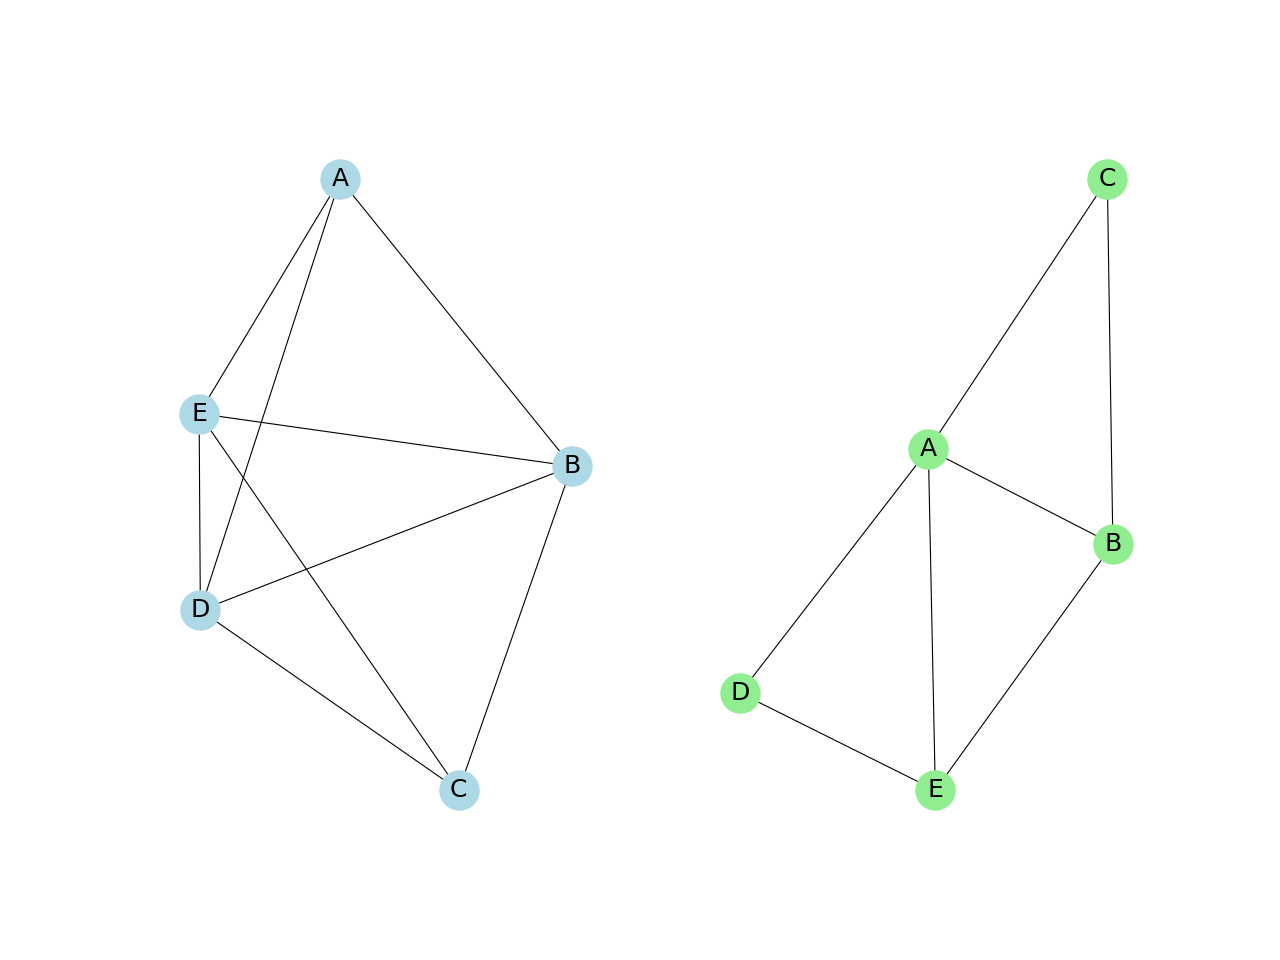
\includegraphics[width=0.7\textwidth]{Graphics/MatrixInNetwork.png}
    \caption{Links ist Netzwerk1 als Graph dargestellt und rechts Netzwerk2}\label{fig:MatrixInNetzwerk}
\end{figure}

Daher können für jegliche Netzwerkanalysen beide Varianten verwendet werden. Jedoch werden in dieser Arbeit überwiegend Graphen zur visuellen Veranschaulichung und Matrizen für jegliche Berechnungen verwendet, da es leichter ist auf die Werte einer Matrix zuzugreifen.\\

Ein soziales Netzwerk ist eine soziale Struktur, die zwischen Akteuren (Einzelpersonen oder Organisationen) besteht. Es zeigt die Art und Weise, wie Menschen und Organisationen durch verschiedene soziale Vertrautheiten verbunden sind, die von zufälligen Bekanntschaften bis hin zu engen familiären Bindungen reichen. Soziale Netzwerke bestehen aus Knotenpunkten und Verbindungen. Die Person oder Organisation, die am Netzwerk teilnimmt, wird als Knoten dargestellt/ bezeichnet. Bindungen sind die verschiedenen Arten von Verbindungen zwischen diesen Knotenpunkten. Bindungen werden nach ihrer Stärke bewertet. Lockere Verbindungen, wie bloße Bekanntschaften, werden als schwache Verbindungen bezeichnet. Starke Verbindungen, wie z. B. Familien oder Cliquen, werden als starke Bindungen bezeichnet \cite{SNADefinition}. Beispiele für soziale Netzwerke sind unsere Gesellschaft, das Internet, unser Gehirn und zelluläre Interaktionen.
Doch welche grundsätzlichen Eigenschaften muss ein Netzwerk erfüllen, um als \textit{soziales Netzwerk} bezeichnet zu werden? 
Sozialwissenschaftler*innen haben drei Arten von Netzwerken untersucht: egozentrische, soziozentrische und systemoffene
Netzwerke. Egozentrische Netze sind Netze, die mit einem einzigen Knoten oder einer einzigen Person verbunden sind \cite{egocentric}. Um als Netze zu gelten, müssen diese Verbindungen nicht nur Auflistungen von Personen oder Organisationen sein, sondern müssen auch Informationen über die Verbindungen zwischen diesen Personen oder Organisationen enthalten. Im allgemeinen Sprachgebrauch, insbesondere, wenn von sozialer Unterstützung die Rede ist, wird jede Liste (dynamische Datenstruktur in der Informatik) als Netzwerk betrachtet. Eine Person, die eine große Anzahl guter Freunde hat, auf die sie sich verlassen kann, besitzt daher im Sprachgebrauch ein großes "Netzwerk". Soziozentrische Netzwerke sind, wie Russell Bernard definiert, Netzwerke in einer Box. Netze mit offenen Systemen hingegen sind Netze, bei denen die Grenzen nicht klar sind, sie liegen nicht in einer Box, zum Beispiel die Verbindungen zwischen Unternehmen, oder die Kette an Auswirkungen, die eine Entscheidung oder eine Erneuerung in beispielsweise technischen Prozessen nachzieht. In gewisser Weise sind dies die interessantesten Netzwerke. Sie sind jedoch am schwierigsten zu untersuchen \cite{charlesKadushin}. 




%*****************************************
%*****************************************
%*****************************************
%*****************************************
%*****************************************